\section{Introduction}

Large language models (LLMs) are foundational to agentic AI applications, such as automated coding assistants~\citep{wang2025openhandsopenplatformai, yang2024sweagentagentcomputerinterfacesenable}, multi-agent workflows~\citep{wang2024mixtureofagentsenhanceslargelanguage, chen2024autoagentsframeworkautomaticagent}, and retrieval systems~\citep{wang2024speculativeragenhancingretrieval, gao2024retrievalaugmentedgenerationlargelanguage}. Unlike basic chatbots, these workloads issue repetitive and predictable inference requests. For instance, multi-agent systems repeatedly perform similar tasks, and reasoning loops~\citep{wang2023selfconsistencyimproveschainthought, madaan2023selfrefineiterativerefinementselffeedback} regenerate similar token sequences. Despite this predictable repetition, existing methods fail to fully exploit recurring patterns, leaving latency as a bottleneck.

A popular strategy for mitigating inference latency is \emph{speculative decoding}~\citep{leviathan23,chen23,specinfer,cai2024medusasimplellminference, bita, draftverify}. While an LLM can only generate one token per forward pass, it can verify {\em multiple} tokens. Leveraging this phenomenon, speculative decoding methods use small ``draft'' models or additional decoding heads to predict multiple candidate tokens, which the LLM then verifies in parallel.

To efficiently handle the long repetitions common in agent-driven applications, speculative decoding methods must satisfy two critical requirements. First, they need to generate draft tokens rapidly and with minimal overhead, enabling maximal exploitation of long speculation lengths. Second, they must do so \emph{adaptively}---only generating more draft tokens when acceptance likelihood is high and fewer tokens when acceptance likelihood is low, to prevent verification from becoming a bottleneck.

However, existing speculative decoding approaches fall short in meeting these dual requirements. Model-based methods can use significant GPU time when speculating long sequences, and can incur memory contention and kernel-level transitions~\citep{sequoia,eagle2} that must be managed carefully. Conversely, existing model-free approaches, such as prompt-lookup decoding (PLD)~\citep{saxena2023prompt}, achieve low overhead and rapid token generation, but typically lack adaptivity. These methods speculate a fixed number of tokens irrespective of acceptance likelihood, leading to wasted computational resources on verifying long and improbable draft sequences.

\begin{figure*}[ht]
\centering
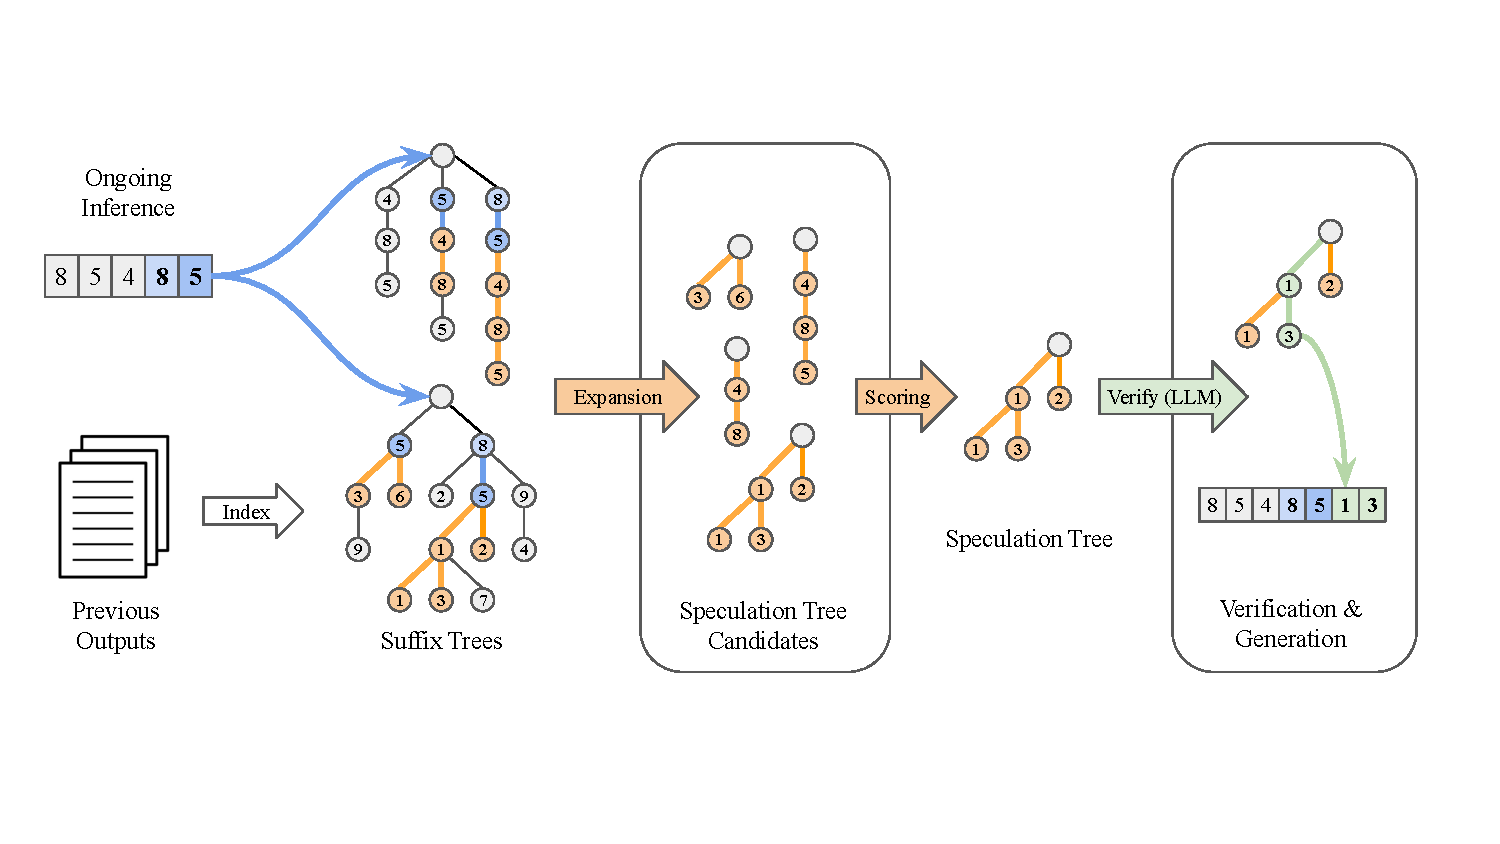
\includegraphics[width=\textwidth,trim={0 80 0 60},clip]{figures/suffix-decoding.pdf}
\caption{Overview of SuffixDecoding's algorithm. Two suffix trees track ongoing inference (top-left) and previous outputs (bottom-left). SuffixDecoding uses these trees to find matching patterns based on recently generated tokens. It constructs a speculation tree (middle) by selecting the most likely continuations, scoring them based on frequency statistics. Finally, the best candidate is verified by the LLM in a single forward pass (right), with accepted tokens (shown in green) being added to the output and used for the next round of speculation.}
\label{fig:suffix-decoding}
\end{figure*}

To address these limitations, we introduce \emph{SuffixDecoding} (Fig~\ref{fig:suffix-decoding}), a model-free speculative decoding method for repetitive, agent-driven workloads. SuffixDecoding uses efficient suffix trees to cache long token sequences from prompts and previous outputs. Each node represents a token, and paths encode previously observed subsequences, enabling rapid pattern matching to identify continuations based on prior occurrences. Draft tokens are generated extremely quickly ($\sim$20 microseconds per token) without GPU overhead.

At each inference step, SuffixDecoding adaptively limits its number of draft tokens based on the length of the pattern match, and uses frequency-based statistics captured within the suffix trees to score and select the best speculation candidate. Longer pattern matches enable confident speculation of longer token sequences, maximizing its effectiveness on agentic workloads, while shorter pattern matches trigger conservative speculation to avoid computational waste. Moreover, SuffixDecoding can seamlessly integrate with existing model-based speculative decoding methods. This flexibility enables a hybrid approach that leverages suffix-tree-based speculation for repetitive, predictable agentic workloads, while exploiting the strengths of model-based speculation methods for open-ended conversational tasks, thus achieving the best of both worlds.

We evaluate SuffixDecoding on two practical agent-driven workloads: SWE-Bench, an LLM-based software engineering benchmark, and AgenticSQL, a proprietary multi-agent pipeline application for SQL generation. We compare with state-of-the-art model-based and model-free speculative decoding methods using Spec-Bench~\citep{xia2024unlockingefficiencylargelanguage}, showing up to 2.8$\times$ faster decoding than EAGLE-2/3~\citep{li2025eagle3scalinginferenceacceleration}, and 1.9$\times$ faster decoding than Token Recycling~\citep{luo2024turningtrashtreasureaccelerating}. For SWE-Bench, we also measured the comprehensive, end-to-end task completion time---including prompt prefilling, token generation, and execution of external actions---and demonstrate speculative speedups of up to 4.5$\times$. These results highlight that SuffixDecoding substantially reduces latency for real-world agentic applications, addressing a critical bottleneck in practical inference scenarios.
